\chapter{Shapley Attribution Charts (Study 11)}
\label{appendix:shapley-charts}

Study~11 charts (Section~\ref{subsec:study-11-shapley-verification}, Tables~\ref{tab:shapley-verification} and~\ref{tab:shapley-source-dominance}).

\begin{figure}[ht!]
    \centering
    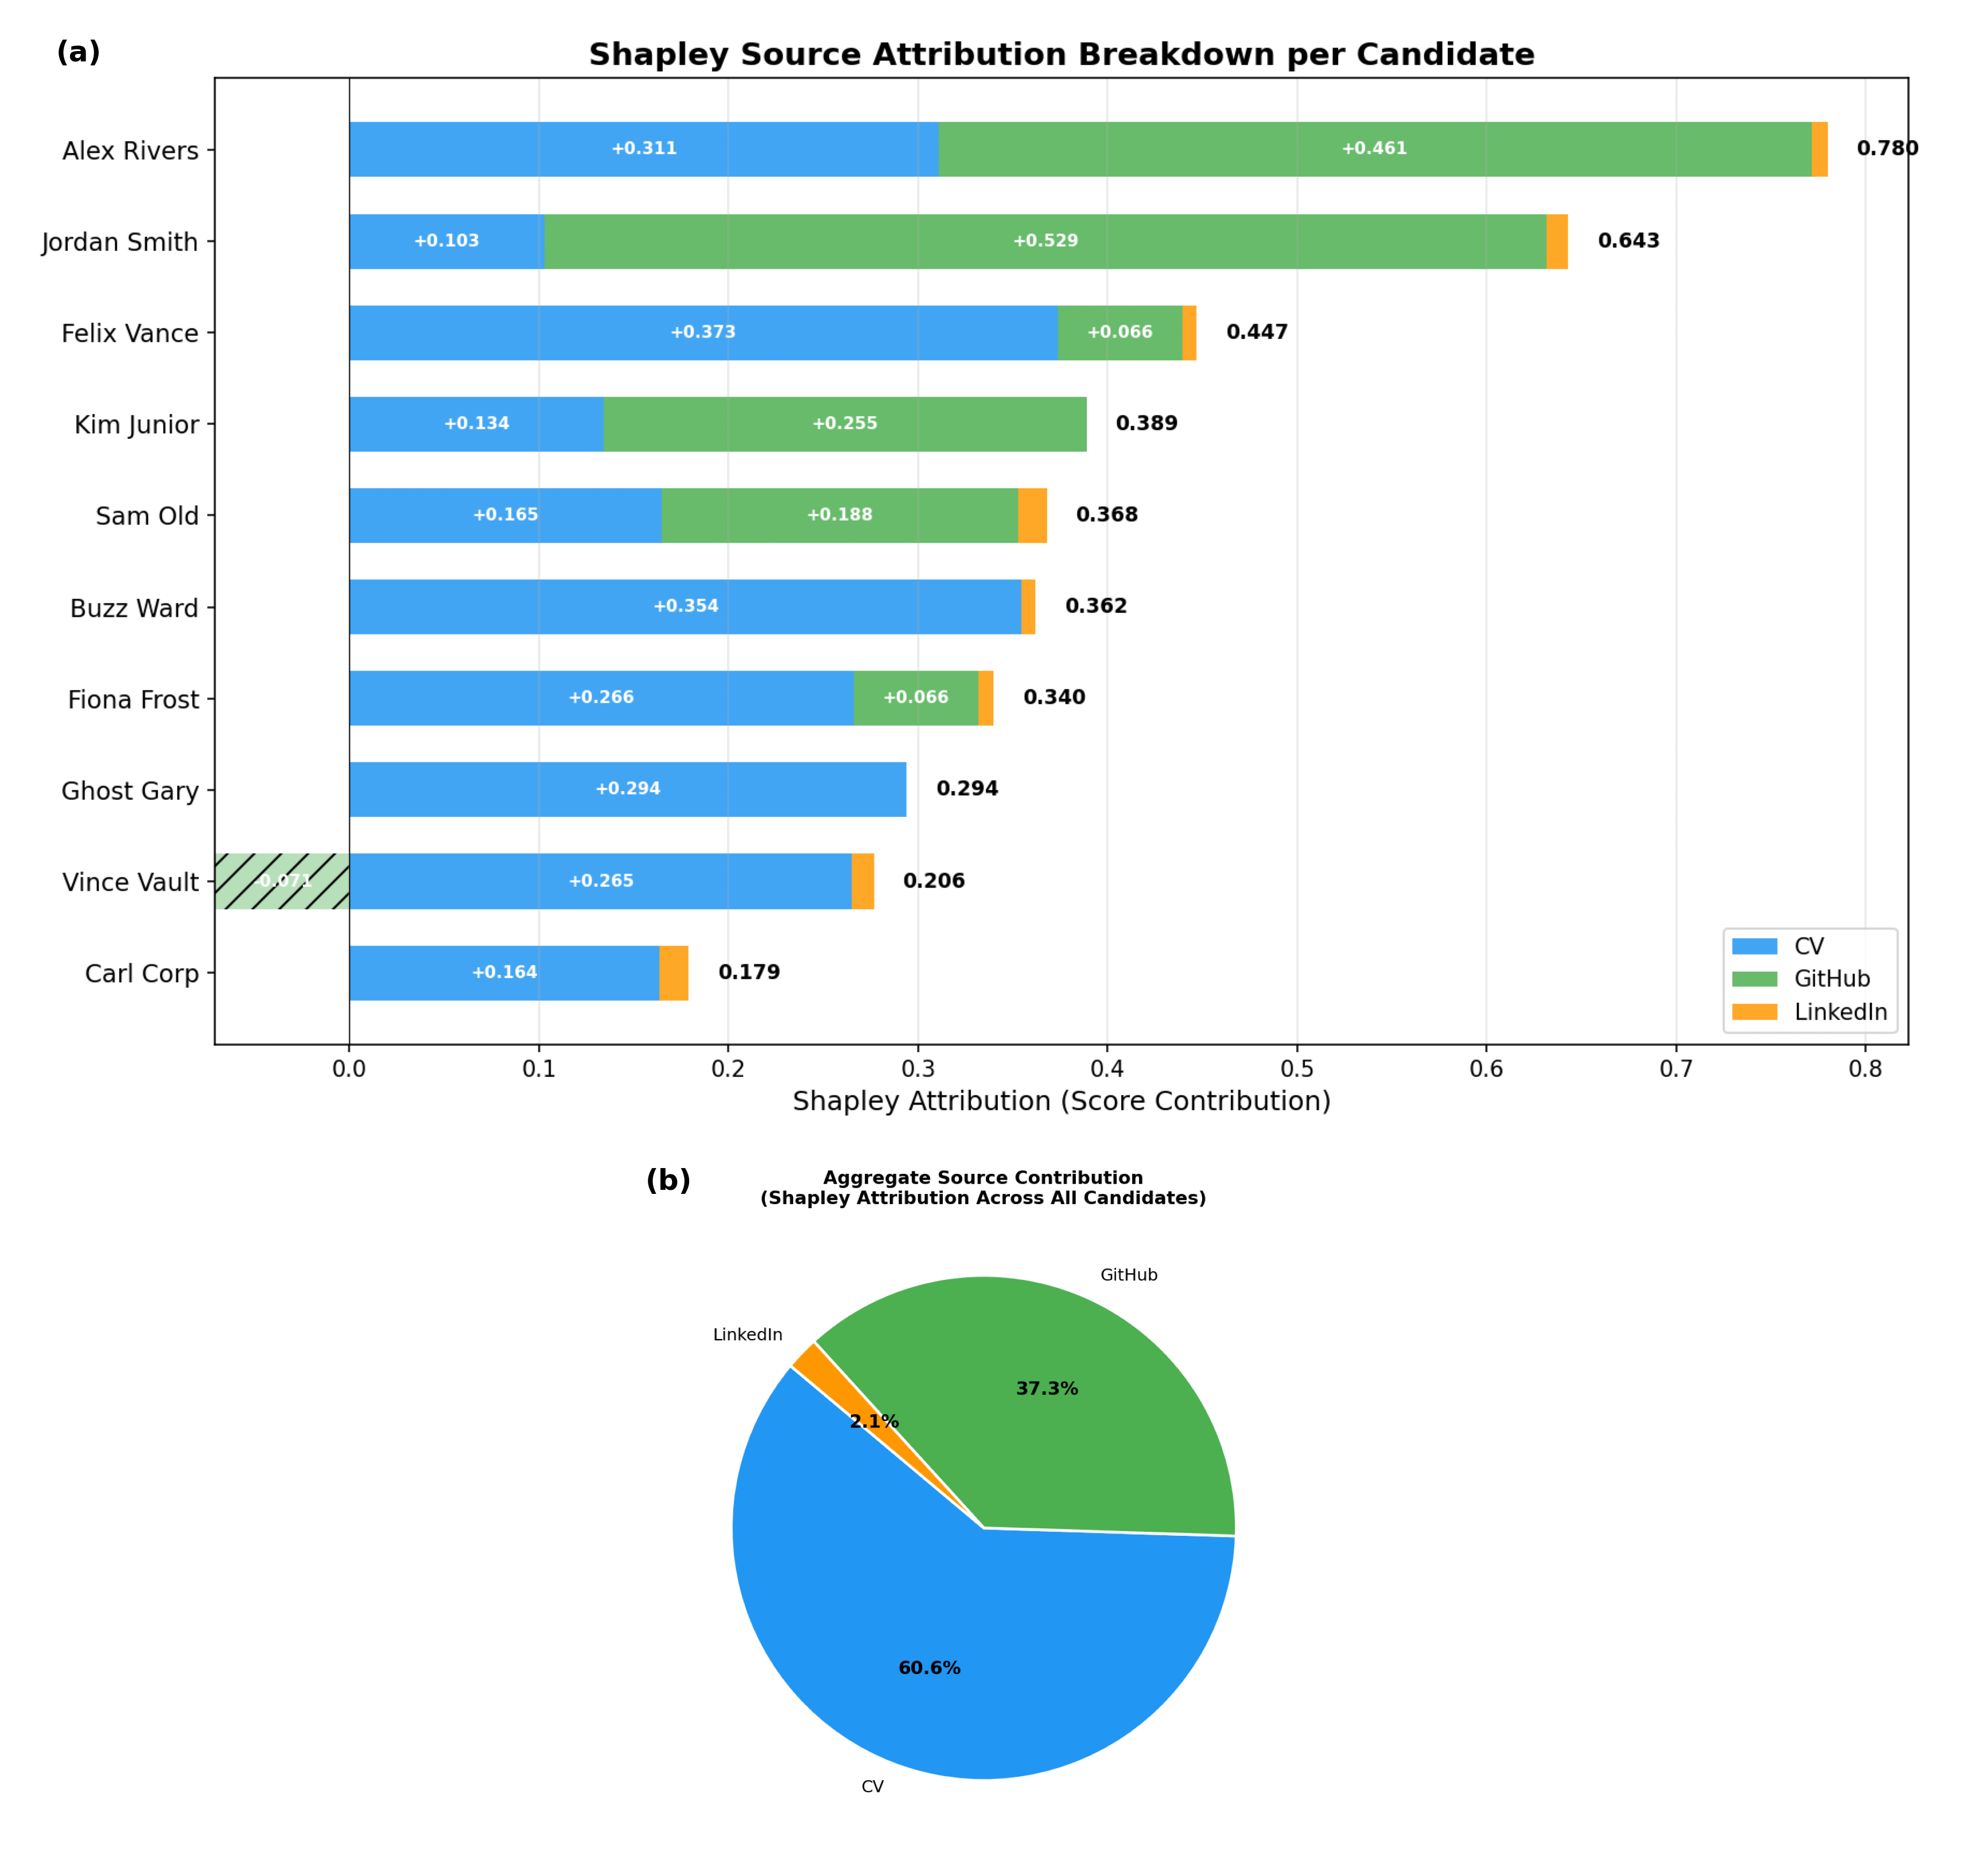
\includegraphics[width=0.95\textwidth]{../evaluation/report_charts/shapley_charts/output/shapley_combined_chart.png}
    \caption[Study~11: Shapley attribution]{Study~11: Shapley attribution with per-candidate breakdown (a) and aggregate source shares (b).}
    \label{fig:shapley-combined}
\end{figure}

\section*{Per-Metric Efficiency Verification}
Table~\ref{tab:per-metric-shapley-verification} demonstrates the per-metric efficiency of the Shapley layer for two randomly selected candidates (Jordan Smith and Felix Vance). As established in Section~\ref{subsec:study-11-shapley-verification}, the efficiency axiom dictates that the sum of the source attributions must perfectly equal the final evaluated score. In these breakdowns, we show that this axiom holds strictly true not only for the candidate's global aggregate score, but for every individual granular metric evaluated by the system.

Notably, Jordan Smith achieves a peak metric score of $0.910$ for both the React and Java requirements, driven entirely by GitHub ($\phi_{\mathrm{GH}} = 0.910$). While the theoretical ``full-evidence'' profile converges to a ceiling of $0.861$ (as demonstrated in Appendix~\ref{appendix:bayesian-fusion-charts}), that ceiling assumes the presence of CV and LinkedIn signals. Because self-claim sources are bounded by a maximum signal of $s=0.8$, they inject a permanent degree of doubt mass (adding to the $\beta$ parameter in the Beta distribution) which mathematically caps the upper bound. Because Jordan Smith had zero CV or LinkedIn claims for these specific skills, his score relied purely on demonstrated evidence ($s=1.0$), allowing him to bypass the self-claim penalty and pierce the theoretical full-evidence ceiling. However, this is an intended feature of the system rather than a flaw: by relying on a single evidence source, Jordan fundamentally retains a higher uncertainty standard deviation ($\sigma$) compared to a multi-source candidate, and his narrow focus results in scoring $0.000$ in several other metrics (such as AWS and Spring Boot), naturally balancing his global aggregate score.

\begin{table}[htbp]
    \centering
    \caption[Study 11: Per-metric Shapley breakdown]{Study 11: Per-metric Shapley verification ($\sum \phi_i = v_m(N)$) for Jordan Smith (left) and Felix Vance (right).}
    \label{tab:per-metric-shapley-verification}
    \scriptsize
    \setlength{\tabcolsep}{2.5pt}
    \begin{minipage}{0.48\textwidth}
        \centering
        \textbf{Jordan Smith} \\[1mm]
        \begin{tabular}{l c c c c c}
            \toprule
            \textbf{Metric} ($m$) & $\phi_{\mathrm{CV}}$ & $\phi_{\mathrm{GH}}$ & $\phi_{\mathrm{LI}}$ & $\sum \phi_i$ & $v_m(N)$ \\ \midrule
            Spring Boot Req. & $0.000$ & $0.000$ & $0.000$ & $0.000$ & $0.000$ \\
            React Req.       & $0.000$ & $0.910$ & $0.000$ & $0.910$ & $0.910$ \\
            AWS Req.         & $0.000$ & $0.000$ & $0.000$ & $0.000$ & $0.000$ \\
            Java Req.        & $0.000$ & $0.910$ & $0.000$ & $0.910$ & $0.910$ \\
            TypeScript Req.  & $0.000$ & $0.830$ & $0.000$ & $0.830$ & $0.830$ \\
            Experience       & $0.250$ & $0.000$ & $0.000$ & $0.250$ & $0.250$ \\
            Projects         & $0.000$ & $0.700$ & $0.000$ & $0.700$ & $0.700$ \\
            Prof. Gravity    & $0.420$ & $0.000$ & $0.300$ & $0.720$ & $0.720$ \\
            Education        & $0.780$ & $0.000$ & $0.000$ & $0.780$ & $0.780$ \\ \bottomrule
        \end{tabular}
    \end{minipage}
    \hfill
    \begin{minipage}{0.48\textwidth}
        \centering
        \textbf{Felix Vance} \\[1mm]
        \begin{tabular}{l c c c c c}
            \toprule
            \textbf{Metric} ($m$) & $\phi_{\mathrm{CV}}$ & $\phi_{\mathrm{GH}}$ & $\phi_{\mathrm{LI}}$ & $\sum \phi_i$ & $v_m(N)$ \\ \midrule
            Spring Boot Req. & $0.710$ & $0.000$ & $0.000$ & $0.710$ & $0.710$ \\
            React Req.       & $0.000$ & $0.000$ & $0.000$ & $0.000$ & $0.000$ \\
            AWS Req.         & $0.710$ & $0.000$ & $0.000$ & $0.710$ & $0.710$ \\
            Java Req.        & $0.710$ & $0.000$ & $0.000$ & $0.710$ & $0.710$ \\
            TypeScript Req.  & $0.000$ & $0.000$ & $0.000$ & $0.000$ & $0.000$ \\
            Experience       & $0.800$ & $0.000$ & $0.000$ & $0.800$ & $0.800$ \\
            Projects         & $0.000$ & $0.700$ & $0.000$ & $0.700$ & $0.700$ \\
            Prof. Gravity    & $0.400$ & $0.000$ & $0.200$ & $0.600$ & $0.600$ \\
            Education        & $0.000$ & $0.000$ & $0.000$ & $0.000$ & $0.000$ \\ \bottomrule
        \end{tabular}
    \end{minipage}
\end{table}

\begin{figure}[ht!]
    \centering
    % Jordan Smith Charts
    \begin{minipage}{0.38\textwidth}
        \centering
        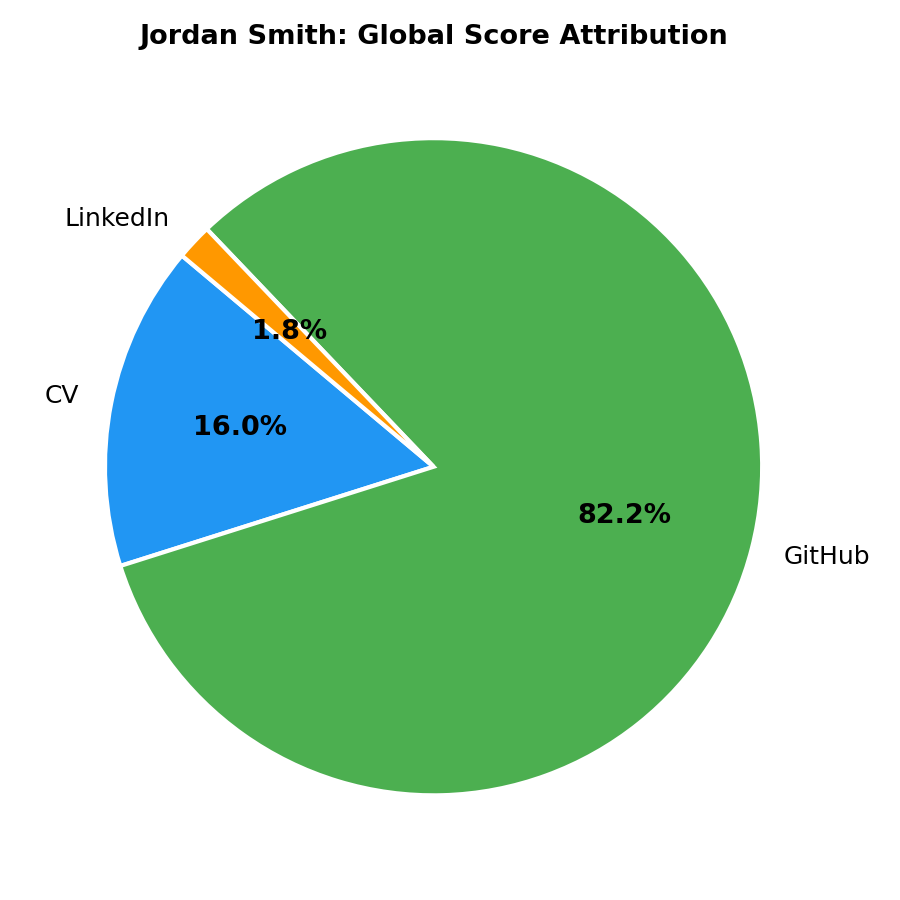
\includegraphics[width=\textwidth]{../evaluation/report_charts/shapley_charts/output/jordan_smith_pie.png}
    \end{minipage}
    \hfill
    \begin{minipage}{0.58\textwidth}
        \centering
        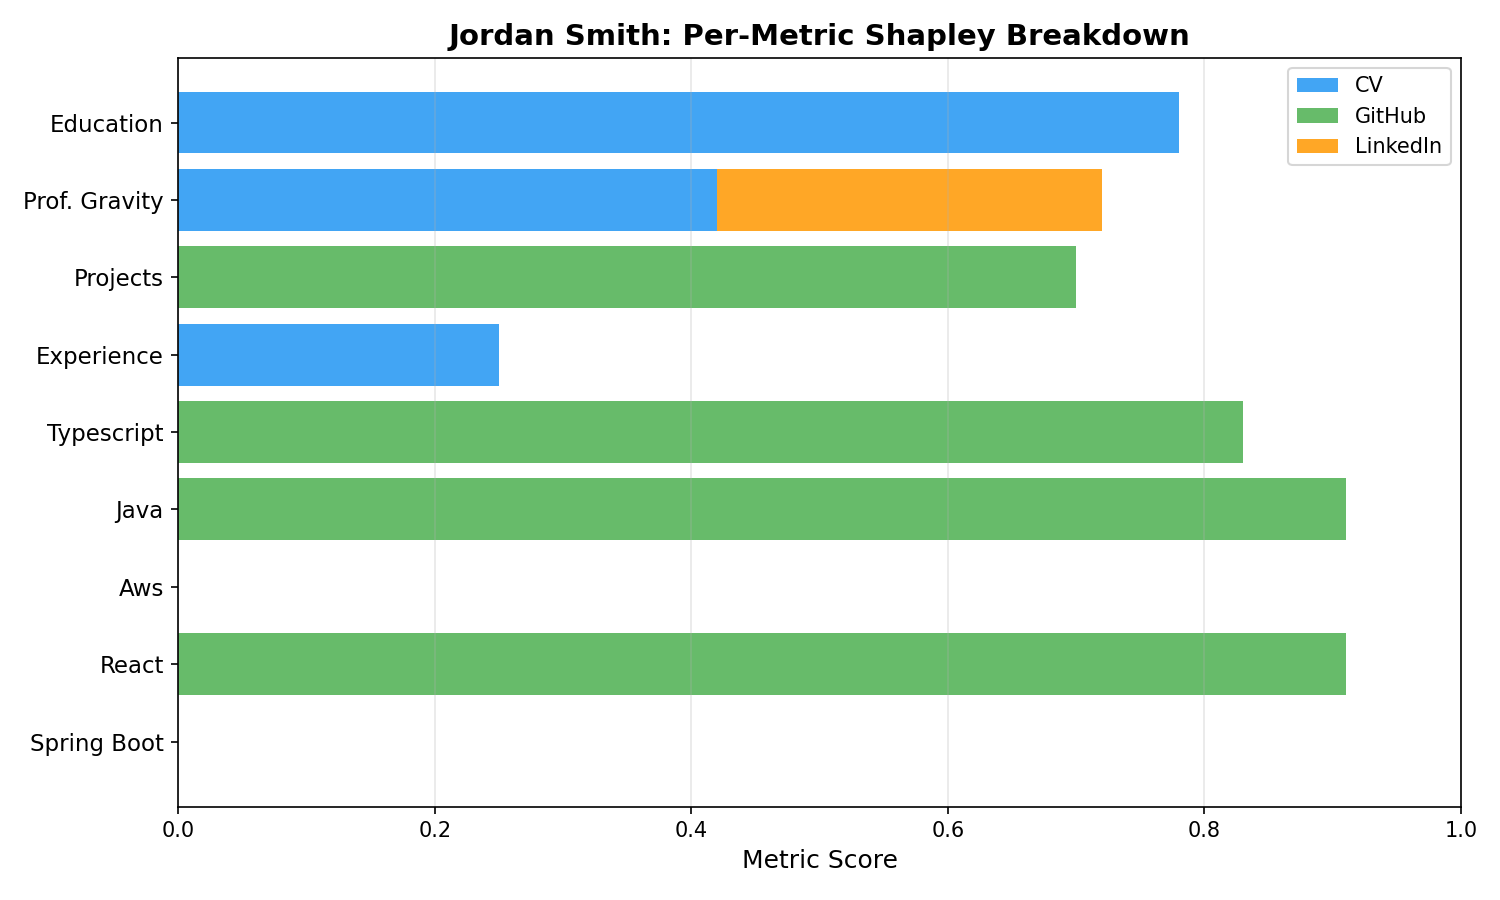
\includegraphics[width=\textwidth]{../evaluation/report_charts/shapley_charts/output/jordan_smith_metrics_bar.png}
    \end{minipage}
    
    \vspace{4mm}
    
    % Felix Vance Charts
    \begin{minipage}{0.38\textwidth}
        \centering
        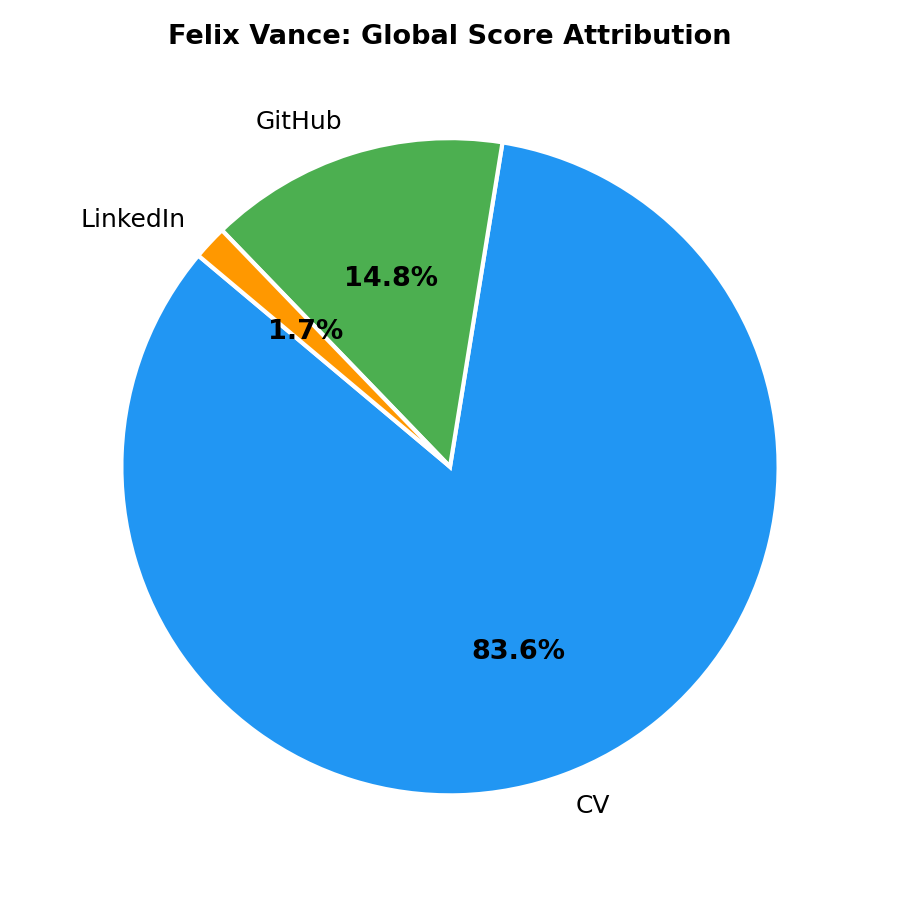
\includegraphics[width=\textwidth]{../evaluation/report_charts/shapley_charts/output/felix_vance_pie.png}
    \end{minipage}
    \hfill
    \begin{minipage}{0.58\textwidth}
        \centering
        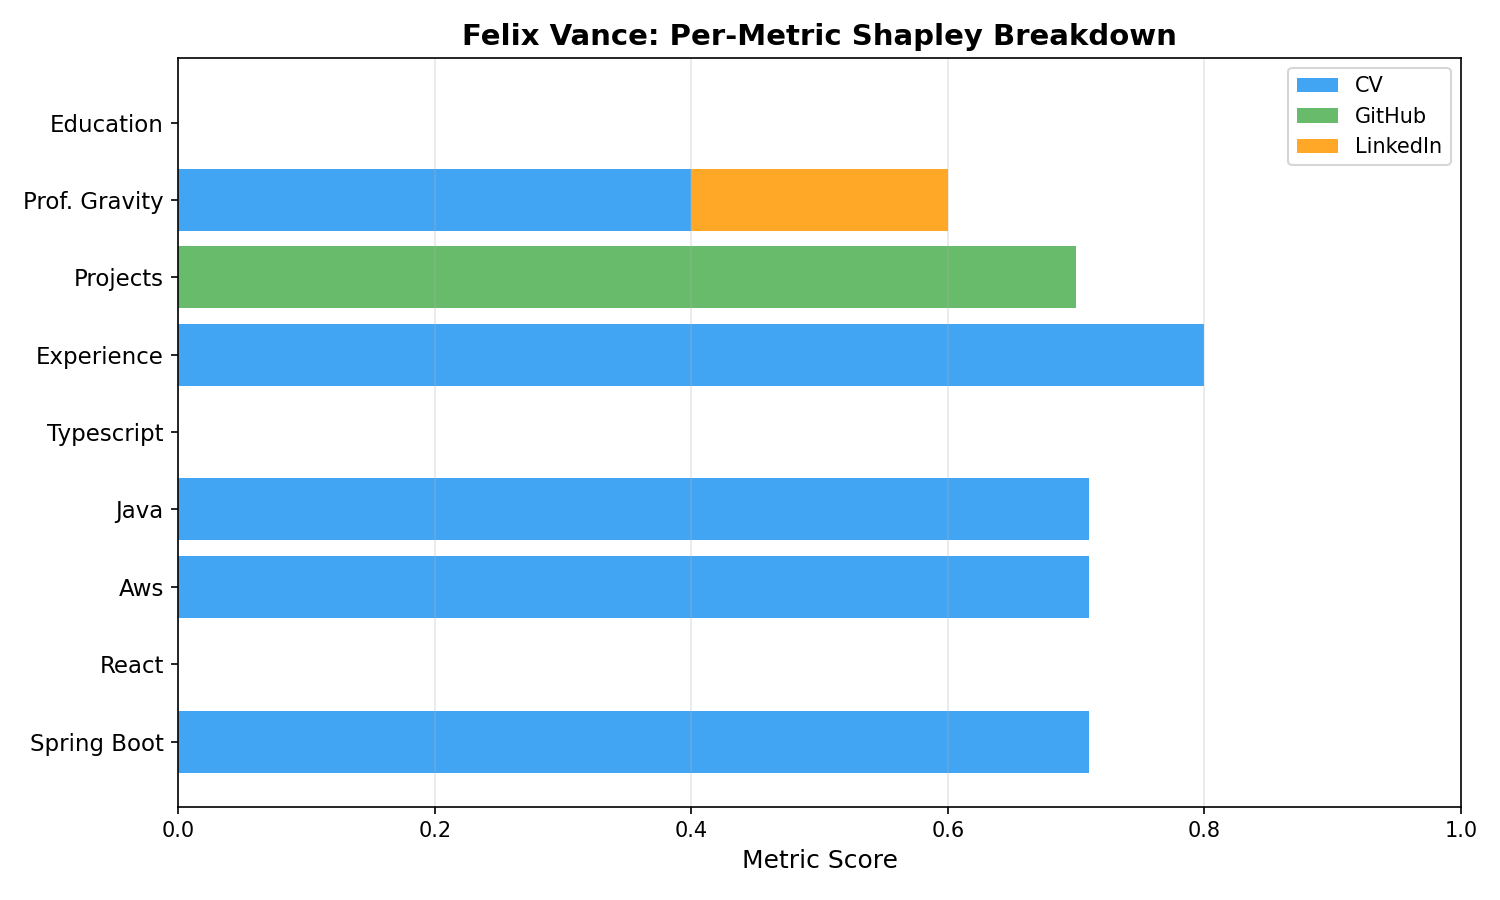
\includegraphics[width=\textwidth]{../evaluation/report_charts/shapley_charts/output/felix_vance_metrics_bar.png}
    \end{minipage}
    \caption[Study 11: Graphical Shapley breakdown]{Study 11: Graphical Shapley breakdown for Jordan Smith (top) and Felix Vance (bottom).}
    \label{fig:shapley-metric-breakdowns}
\end{figure}
